\section{Feature extractor design}
Our feature vector takes as input a set of vectors with three values; an x-co\"ordinate, a y-co\"ordinate and a bit (0 or 1) denoting whether the mouse button was pressed. The size of this set of vectors is in the order of hundreds: the location is measured 50 times per second, so a 3 second timeframe is represented by 150 vectors.

The output of the feature extractor is a set of 

% Code
\begin{minted}[mathescape, linenos, numbersep=5pt, frame=lines, framesep=2mm, tabsize=4, numberblanklines=true, breaklines=true]{matlab}
>> test
percentage of ones: 73.41%
percentage of twos: 26.59%
\end{minted}


\begin{figure}[H]
	\centering
	\begin{minipage}{.45\textwidth}
		\centering
		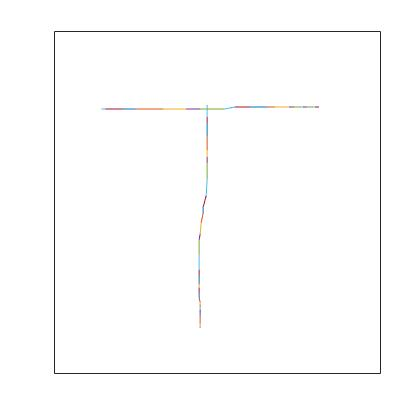
\includegraphics[width=.7\linewidth]{images/T_drawing}
		\captionof{figure}{Drawing of capital T (first line down, then line to right)}
		\label{fig:features_T}
	\end{minipage}%
	\begin{minipage}{.45\textwidth}
		\centering
		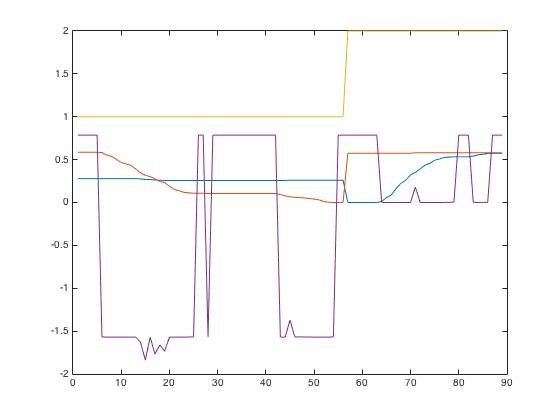
\includegraphics[width=.99\linewidth]{images/T_graph}
		\captionof{figure}{Extracted features, 1 is line down, 2 is line to the right}
		\label{fig:features_plus}
	\end{minipage}
\end{figure}
\begin{figure}[H]
	\centering
	\begin{minipage}{.45\textwidth}
		\centering
		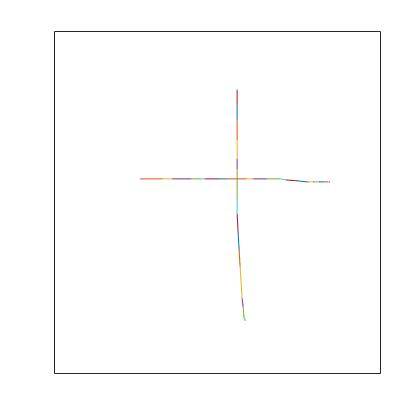
\includegraphics[width=.7\linewidth]{images/+_drawing}
		\captionof{figure}{Features of + sign (first line down, then line to right)}
		\label{fig:features_T}
	\end{minipage}%
	\begin{minipage}{.45\textwidth}
		\centering
		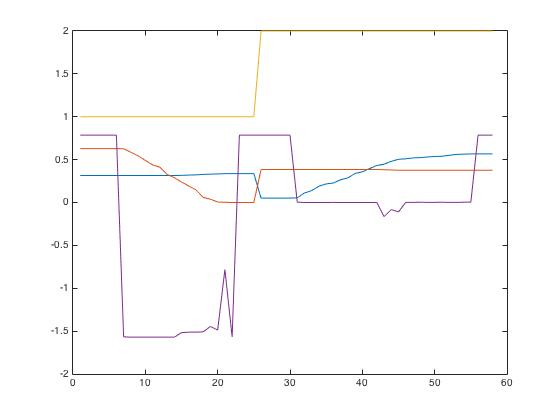
\includegraphics[width=.99\linewidth]{images/+_graph}
		\captionof{figure}{Extracted features, 1 is line down, 2 is line to the right}
		\label{fig:features_plus}
	\end{minipage}
\end{figure}